\documentclass[12pt]{article}
\usepackage[utf8]{inputenc}

\usepackage{polski}
\usepackage{pgfplots}
\usepackage{booktabs} 

\begin{document}
 
\begin{titlepage}
\begin{center}

\includegraphics[scale=1.0]{./Pwr_logo/logo_PWr_2.png}
\\
\vspace{1.5cm}
{\Huge Marcin Karasiewicz}
\\
\begin{Large}
\vspace{1.0cm}
Projektowanie algorytmów \\ i metody sztucznej inteligencji \\
\vspace{1.0cm}
Algorytmy sortowania
\end{Large}
\end{center}
\newpage
\tableofcontents 

\end{titlepage}
\newpage
 
\section{Algorytm Merge Sort }
\subsection{Opis}
\subsection{Tabela pomiarów}

\begin{center}
\begin{tabular}{ccccc}  
\\
\toprule
Rozmiar[n] & \multicolumn{4}{c}{Czas[s]} \\
\cmidrule(r){2-5}
 & Losowe & Posortowane & O-Posortowane & Identyczne \\
\midrule
10       & 0.000000   & 0.080062 & 0.080062  & 0.000000 \\
100      & 0.000006   & 0.080062 & 0.080062  & 0.000004 \\
1000     & 0.000060   & 0.080062 & 0.080062  & 0.000044 \\
10000    & 0.001351   & 0.080062 & 0.080062  & 0.001476 \\
100000   & 0.010007   & 0.080062 & 0.080062  & 0.009358 \\
1000000  & 0.077865   & 0.080062 & 0.080062  & 0.080062 \\
10000000 & 0.838566   & 0.080062 & 0.080062  & 0.080062 \\
\bottomrule
\end{tabular}
\end{center}

\subsection{Wykres}

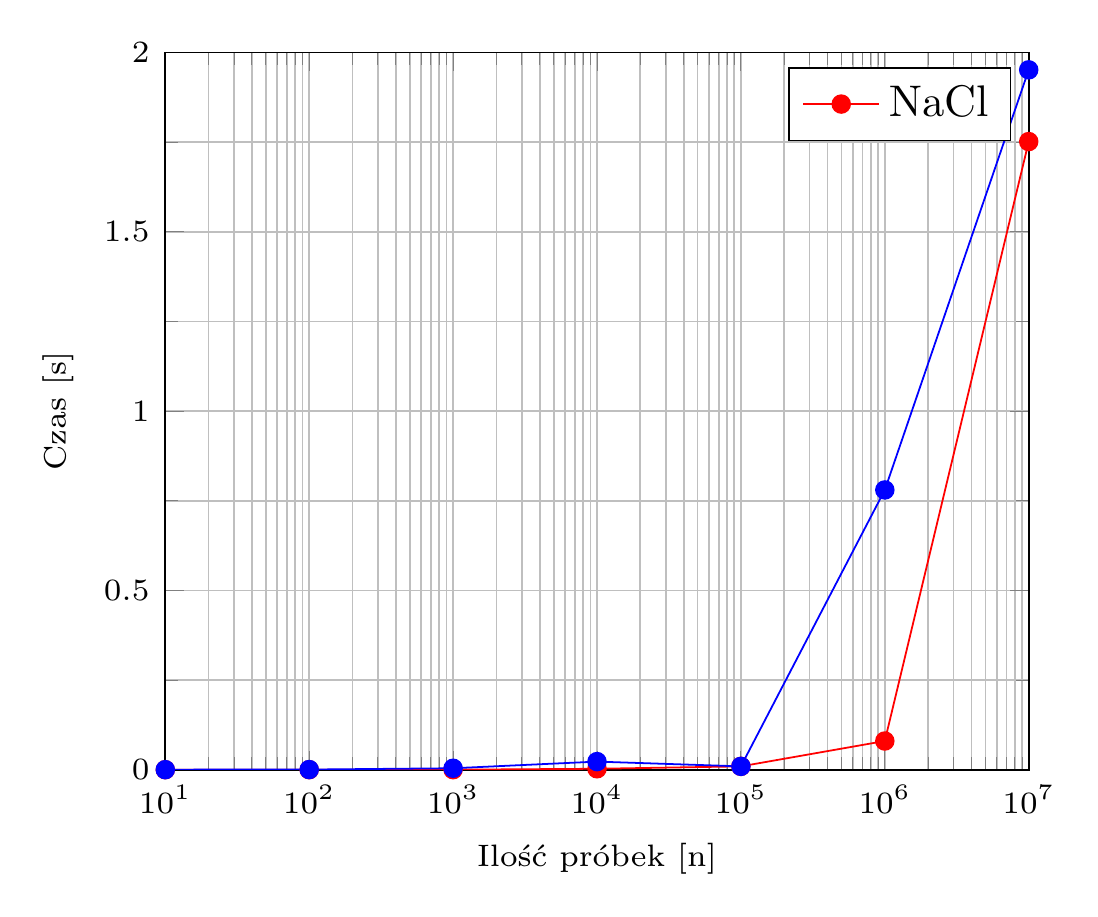
\begin{tikzpicture}[scale=1.6]
\\
\begin{axis}[
	xmode = log,
	xlabel={Ilość próbek [n]},
	ylabel={Czas [s]},
	xmin=10,xmax=10000000,
	ymin=0,ymax=2,
	label style={font=\scriptsize},
	tick label style={font=\scriptsize},
	grid = both,
	minor y tick num=1
]

\addplot[color=red,mark=*]
coordinates {
(10,0.000001 )
(100,0.000004)
(1000,0.000110)
(10000,0.002659)
(100000,0.009358)
(1000000,0.080062)
(10000000,1.751383)
};

\addplot[color=blue,mark=*]
coordinates {
(10,0.000201 )
(100,0.000504)
(1000,0.004110)
(10000,0.022659)
(100000,0.009358)
(1000000,0.780062)
(10000000,1.951383)
};

\legend{NaCl}
\end{axis}
\end{tikzpicture}

\section{Algorytm Quick Sort }
\subsection{Opis}
\subsection{Tabela pomiarów}

\begin{center}
\begin{tabular}{ccccc} 
\\ 
\toprule
Rozmiar[n] & \multicolumn{4}{c}{Czas[s]} \\
\cmidrule(r){2-5}
 & Losowe & Posortowane & O-Posortowane & Identyczne \\
\midrule
10       & 0.000000   & 0.080062 & 0.080062  & 0.000001 \\
100      & 0.000006   & 0.080062 & 0.080062  & 0.000004 \\
1000     & 0.000088   & 0.080062 & 0.080062  & 0.000110 \\
10000    & 0.000874   & 0.080062 & 0.080062  & 0.002659 \\
100000   & 0.008497   & 0.080062 & 0.080062  & 0.009358 \\
1000000  & 0.094046   & 0.080062 & 0.080062  & 0.080062 \\
10000000 & 50.751383  & 0.080062 & 0.080062  & 0.080062 \\
\bottomrule
\end{tabular}
\end{center}

\subsection{Wykres}

\section{Algorytm Heap Sort }
\subsection{Opis}
\subsection{Tabela pomiarów}

\begin{center}
\begin{tabular}{ccccc} 
\\ 
\toprule
Rozmiar[n] & \multicolumn{4}{c}{Czas[s]} \\
\cmidrule(r){2-5}
 & Losowe & Posortowane & O-Posortowane & Identyczne \\
\midrule
10       & 0.000000   & 0.080062 & 0.080062  & 0.000001 \\
100      & 0.000006   & 0.080062 & 0.080062  & 0.000004 \\
1000     & 0.000088   & 0.080062 & 0.080062  & 0.000110 \\
10000    & 0.000874   & 0.080062 & 0.080062  & 0.002659 \\
100000   & 0.008497   & 0.080062 & 0.080062  & 0.009358 \\
1000000  & 0.094046   & 0.080062 & 0.080062  & 0.080062 \\
10000000 & 50.751383  & 0.080062 & 0.080062  & 0.080062 \\
\bottomrule
\end{tabular}
\end{center}

\subsection{Wykres}

\section{Algorytm Hybrid Sort }
\subsection{Opis}
\subsection{Tabela pomiarów}

\begin{center}
\begin{tabular}{ccccc}  
\\
\toprule
Rozmiar[n] & \multicolumn{4}{c}{Czas[s]} \\
\cmidrule(r){2-5}
 & Losowe & Posortowane & O-Posortowane & Identyczne \\
\midrule
10       & 0.000000   & 0.080062 & 0.080062  & 0.000001 \\
100      & 0.000006   & 0.080062 & 0.080062  & 0.000004 \\
1000     & 0.000088   & 0.080062 & 0.080062  & 0.000110 \\
10000    & 0.000874   & 0.080062 & 0.080062  & 0.002659 \\
100000   & 0.008497   & 0.080062 & 0.080062  & 0.009358 \\
1000000  & 0.094046   & 0.080062 & 0.080062  & 0.080062 \\
10000000 & 50.751383  & 0.080062 & 0.080062  & 0.080062 \\
\bottomrule
\end{tabular}
\end{center}

\subsection{Wykres}

\section{Wnioski}


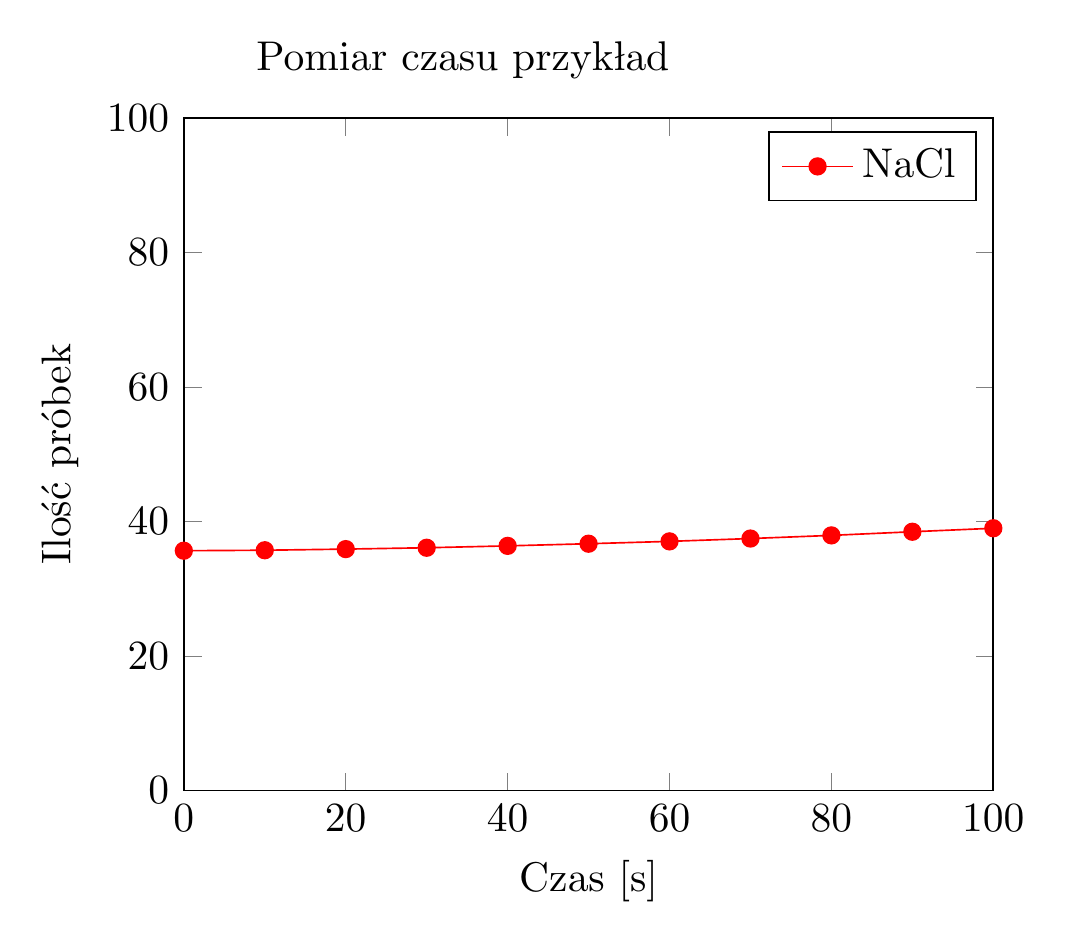
\begin{tikzpicture}[scale=1.5]
\begin{axis}[
title={Pomiar czasu przykład},
title style={text width=16em},
xlabel={Czas [s]},
ylabel={Ilość próbek},
xmin=0,xmax=100,
ymin=0,ymax=100,
]

\addplot[color=red,mark=*]
coordinates {
(0,35.65)
(10,35.72)
(20,35.89)
(30,36.09)
(40,36.37)
(50,36.69)
(60,37.04)
(70,37.46)
(80,37.93)
(90,38.47)
(100,38.99)
};

\legend{NaCl,CuSO$_4\cdot$5H$_2$O}
\end{axis}
\end{tikzpicture}

\end{document}